\section{Architecture of the implemented PoC}
\label{sec:architecture}

\subsection{Three packages, one direction}

The PoC is three independent Python packages, each built as its own \code{uv} project, connected
by a strict one-way dependency chain: \repo{residual/} $\rightarrow$ \repo{reconstruct/}
$\rightarrow$ \repo{gapmap/}. \evobs{} Within that chain, a package may import stdlib,
\code{pydantic}, and any package to its left, and nothing else. \repo{reconstruct/} also depends on
\code{httpx}, \code{openai}, \code{tldextract}, and \code{pypdf} for what only it does: fetching,
model calls, and URL and PDF parsing. \repo{gapmap/}'s one model call goes over stdlib
\code{urllib}, adding nothing beyond \code{residual}. Both rules are checked by a plain,
hand-written \code{pytest} architecture test that walks the import graph with Python's \code{ast}
module. The architecture decision records (ADRs) name this check \code{pytest-archon}, but this repository does not
install that package; the check runs in code, not just as a design-document statement (decisions
\href{https://github.com/AdamKrysztopa/edu_proj/blob/main/docs/architecture/decisions/0006-residual-accounting-core.md}{0006},
\href{https://github.com/AdamKrysztopa/edu_proj/blob/main/docs/architecture/decisions/0007-reconstruction-pipeline.md}{0007},
\href{https://github.com/AdamKrysztopa/edu_proj/blob/main/docs/architecture/decisions/0008-gapmap-methodology-gap-candidates.md}{0008, proposed}).
A fourth package, \repo{instrument/} (the frozen Validation Track A apparatus,
\cref{sec:scope}), sits outside this chain entirely: no NOW package imports it, and it imports
none of them. \Cref{fig:architecture} shows the data flow across all three; \cref{tab:packages}
summarizes each package.

\begin{figure}[tbp]
  \centering
  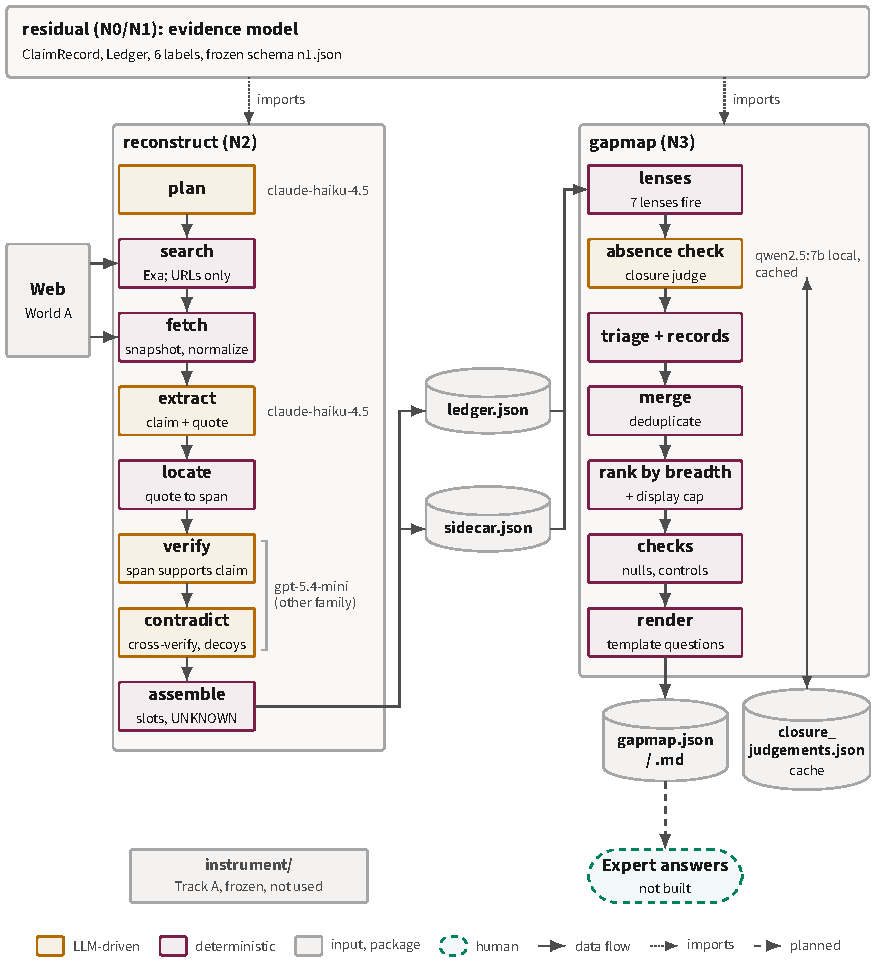
\includegraphics{figures/pdf/fig04_architecture.pdf}
  \caption[Implemented PoC architecture]{The implemented PoC: three packages, one direction of
  dependency, the artifacts written between them, and the external models each stage calls. Solid
  boxes and arrows exist in code and are offline-tested; most have also completed on a live run,
  but cross-verify and the current decoy stage have not completed live without a defect
  intervening (\cref{sec:not-demonstrated}). The human step at the far right does not exist yet in
  the PoC.}
  \label{fig:architecture}
\end{figure}

\begin{table}[tbp]
  \centering
  \small
  \caption{The three NOW packages: purpose, size, and tests. Test counts are from running each
  suite live on 2026-09-29 (\code{uv run --directory <pkg> pytest -q}), not from a grep-based
  count of test functions in the source.}
  \label{tab:packages}
  \begin{tabularx}{\linewidth}{@{}lp{3.1cm}rrX@{}}
    \toprule
    Package & Purpose & LOC & Tests (run) & Runtime dependencies \\
    \midrule
    \repo{residual/} & Typed evidence model: claim record, six epistemic labels, gates &
      1{,}281 & 268 & stdlib + \code{pydantic} only \\
    \repo{reconstruct/} & Populate a ledger from the open web, with verified provenance &
      4{,}803 & 416 & + \code{residual}; \code{httpx}, \code{openai}, \code{tldextract},
      \code{pypdf} \\
    \repo{gapmap/} & Read a ledger, propose ranked gap candidates and expert questions &
      2{,}986 & 172 & + \code{residual}; local Ollama over \code{urllib} \\
    \bottomrule
  \end{tabularx}
\end{table}

\subsection{\code{residual/}: the evidence model (N0/N1)}

\repo{residual/} defines the typed record of a claim, its provenance, and its epistemic label; it
is the domain-neutral core that N2 and N3 both write to and read from. \evobs{} It depends at
runtime only on \code{pydantic}, checked by the test
\code{test_modules_import_only_stdlib_pydantic_and_residual}. Nine modules (counting \code{__init__.py}, as for the other two packages) total 1{,}281 lines,
covering the claim record, its provenance types, the ledger, the evidential gate, the N1 feature
definitions, and the freeze mechanism. The module-by-module inventory is in \cref{app:reproduce};
the claim record, labels, and provenance chain are detailed in \cref{sec:evidence-model}.

\subsection{\code{reconstruct/}: the reconstruction pipeline (N2)}

\repo{reconstruct/} populates an N1 ledger for one \code{(domain, task)} pair from the open web,
with real provenance. Ten modules, 4{,}803 lines, 416 tests, none of which calls a live model or
the network (fakes only); a live run needs \code{python -m reconstruct.run --live} with a hard
\code{--max-usd}. The pipeline (\repo{reconstruct/src/reconstruct/run.py},
\repo{reconstruct/src/reconstruct/evidence.py}) is one \code{reconstruct(domain, task, ...)} call,
strictly one-way, with no agent loop:

\begin{enumerate}[noitemsep]
  \item \textbf{plan} -- propose 3--6 areas with search queries.
  \item \textbf{search / fetch} -- search via an OpenRouter web plugin; fetch, normalize, and hash
    each document once into a content-addressed snapshot store.
  \item \textbf{extract} -- one model call per document, pulling schema-bound candidate assertions.
  \item \textbf{locate} -- the extractor's quote must occur verbatim, after normalization, in the
    document's own normalized text, or the extraction produces no \code{Evidence} at all.
  \item \textbf{independence} -- union-find over fetched documents. Two documents merge into one
    cluster when their registrable domain matches (a hand-listed set of multi-organization
    domains, e.g.\ \code{arxiv.org}, is grouped by full host instead), or when their 5-shingle
    overlap is at least 0.5. Corroboration is counted per independent cluster.
  \item \textbf{verify} -- a second model, from a different model family than the extractor's,
    judges support on an annotated window around the located span.
  \item \textbf{cross-verify} -- claims sharing an area are cross-checked against topically-near
    claims from a different independence cluster; a contradicting verdict becomes a
    \code{Contradiction} record.
  \item \textbf{slot status and decoys} -- each (area, probe) pair is marked covered, thin,
    unknown, unverified, or unexamined. A \code{ClaimRecord} with no evidence enters the ledger
    only under \code{unknown}: searched, fetched, and fully verified, with nothing found. Decoy
    mutations (number, negation, scope) estimate a false-accept rate for the verifier.
\end{enumerate}

\repo{reconstruct/models.json} configures planner, extractor, and baseline as
\code{anthropic/claude-haiku-4.5} (family anthropic) and the verifier as \code{openai/gpt-5.4-mini}
(family openai), all served through one OpenRouter backend. The verifier's family must differ from
the extractor's, checked in code, so no claim can move off \emph{pending}/\emph{synthetic} on a
self-verification.

A real completed run (\repo{reconstruct/runs/20260928T133336Z-59ec876b3d7e/}, domain
\enquote{industrial machine maintenance}, task \enquote{PLC intermittent-fault diagnosis}) produced
375 claims: \code{literature_supported} 321, \code{synthetic_extrapolation} 49,
\code{unknown} 5. It drew on 35 fetched sources across 27 independent clusters, for a total cost of
\$0.679 across 473 logged model and search calls. \evobs{} This run left no claim pending. But
neither cross-verify nor the current decoy stage has completed on any live run without a defect
getting in the way. The one run that exercised both, GDPR v2
(\repo{reconstruct/runs/20260928T145943Z-bc1cc9a30a02/}), hit a provider-error defect (since fixed,
\cref{app:defects} row EL10) that left 140 of 366 evidence items pending. That is why 305 of its
523 claims read \code{synthetic\_extrapolation}. That run is not N3-admissible on its own
(\cref{app:claims}, row E23).

\subsection{\code{gapmap/}: the methodology-guided gap map (N3)}

\repo{gapmap/} reads one N2 ledger and proposes gap \emph{candidates}: it never writes a
hypothesis back into a ledger as a claim, and its scores never feed a gate as a criterion. Twelve
modules, 2{,}986 lines, 172 tests, all offline against a fake judge; the CLI replays a committed
judge cache by default. Seven methodology lenses (\code{lenses.py}) fire over criterion-labeled
claims only, each looking for a different missing element:
\begin{itemize}[noitemsep]
  \item \textbf{DISC} -- a judged term attached to multiple claims, no discriminating case;
  \item \textbf{DIAG} -- rival causes with no distinguishing sign;
  \item \textbf{SEL} -- a selection rule with no stated criterion;
  \item \textbf{HEDGE} -- a hedged rule with no exception stated;
  \item \textbf{GUARD} -- an error-avoidance step with no named check;
  \item \textbf{WHY} -- a procedure with no stated rationale;
  \item \textbf{RESULT} -- a test with no stated interpretation.
\end{itemize}
A fired candidate is judged for closure by \code{semantic.judge_candidate} against retrieved
sentences from the same ledger. It is then assembled into a three-tier \code{Record}
(\code{observed_evidence}, \code{inferred_gap}, \code{hypothesis}) and ranked by breadth, not by a
confidence calibrated against any gold (\cref{sec:evidence-model,sec:n3}).

\evobs{} The closure judge is \code{qwen2.5:7b-instruct}, served by a \textbf{local Ollama} instance at
zero cost, chosen because its model family (local) differs from both the ledger's extractor
(anthropic) and verifier (openai) families. This is a decision 0008 requirement, checked by code
review rather than by a test. Judgments are cached to \code{research/n3/<run>/closure_judgements.json},
keyed by \code{sha256(model_id, prompt)}. The CLI's default mode raises an error naming
\code{--judge ollama} on a cache miss, instead of silently calling the network, so a default run
and the test suite both touch no network at all.

\subsection{Determinism, replay, and budget}

Each package's reproducibility guarantee matches what it can and cannot control. \evobs{}
\repo{residual/} is pure, deterministic \code{pydantic} validation with no model or network call.
\repo{reconstruct/} is not deterministic end to end --- it makes live web and live model calls. But
every criterion-labeled claim traces to a byte-fixed snapshot span (\cref{sec:evidence-model}), and
every call is logged, even on failure. \repo{gapmap/} is fully offline by default: its one
model call is cached and replayed by content hash, so a default run and \code{pytest} touch no
network; only \code{--judge ollama} adds new cache entries.

A budget check accumulates cost \emph{before} each call and raises before overspending, writing the
three output files with \code{complete=False} rather than truncating silently. This is a real
constraint, not a theoretical one: N2's post-fix live re-check (E-LIVE v3) never got past its
first call. It was blocked by an exhausted \$5/week OpenRouter key, a provider-side limit
(HTTP 403), not by the code's own check firing. Failed calls are counted per task, making a loss
visible in \code{sidecar.json}. The \code{complete} flag itself, though, is computed independently
of that count, so a run can still read \code{complete=True} after calls have failed. The E-LIVE v2
defect (\cref{app:defects}, row EL10) was exactly this gap. \code{gapmap} narrows the equivalent
risk on its own side: a malformed or out-of-range judge answer is routed to its own retrieval-gap
category, \code{RG-UNDECIDED}, never silently treated as \enquote{open}. This was the fix for a
defect found by adversarial review (\cref{app:defects}, row L7). Module inventories and the budget
and freeze mechanisms' exact fields are in \cref{app:reproduce}.
